\documentclass{hotnets15}

\usepackage{times}  
\usepackage{epsfig}
%\usepackage[TABBOTCAP]{subfigure}
\usepackage{tabularx}
\usepackage{graphicx} 
\usepackage{color}
\usepackage{xspace}
%\usepackage{thumbpdf}
\usepackage{listings}
\usepackage{verbatim}
\usepackage[pdfpagelabels=false]{hyperref}
\usepackage{booktabs}
\usepackage{colortbl}
\urlstyle{rm}

\usepackage{microtype}

\hypersetup{pdfstartview=FitH,pdfpagelayout=SinglePage}

\setlength\paperheight {11in}
\setlength\paperwidth {8.5in}
\setlength{\textwidth}{7in}
\setlength{\textheight}{9.25in}
\setlength{\oddsidemargin}{-.25in}
\setlength{\evensidemargin}{-.25in}

%%%  New commands
\newcommand{\Section}[1]{\hyperref[#1]{Section~\ref*{#1}}}
\newcommand{\sk}{\mathit{sk}}
\newcommand{\pk}{\mathit{pk}}
\newcommand{\DD}{\textrm{D}}

\begin{document}

\conferenceinfo{HotNets 2015} {}
\CopyrightYear{2015}
\crdata{X}
\date{}

%%%%%%%%%%%% THIS IS WHERE WE PUT IN THE TITLE AND AUTHORS %%%%%%%%%%%%

\title{The Case for Self-Incentivizing Networks}

\author{Paper \#36 (7 pages)}

\maketitle

%\thispagestyle{empty}

\subsection*{Abstract}
We argue that computer networks should be made ``self-incentivizing'':
designed so that anybody may contribute incremental capacity and be
rewarded for it. In such a scheme, endpoints express their demand in
terms of a price, not just for ``bandwidth,'' but effectively by
bidding on each packet they want transmitted. This creates a market
incentive to build out capacity where the network needs it most.

Our position is that this kind of mechanism---one where ``paid
priorization'' is celebrated instead of banned, and anybody may be an
ISP-for-a-day---is the missing piece necessary to revive
almost-successful systems of the recent past, such as urban mesh
networks, and foster more innovation and growth in last-mile Internet service.

Would such a system actually work? We evaluated, in simulation, the
stability and performance of a simple market-based congestion-control and queue-management
policy. In these experiments, users bid for
transmission opportunities in a logically-centralized order book and
resell them to one another. In a model where users behave ``nicely,''
this distributed-bidding scheme was sufficient to realize schedules
that closely approximated the shortest-remaining-time-first
schedule.

\section{Introduction}

\label{sec:intro}

On June 12, 2015, the Federal Communications Commission's Open
Internet rules went into effect. In pursuit of what's commonly known
as ``net neutrality,'' the agency bans ``retail'' Internet service
providers from ``blocking,'' ``throttling,'' or ``paid
prioritization'' of traffic across their networks~\cite{openinternet}.

The ``paid priorization'' rule protects third-party
content providers who aren't transit customers or peers of the
ISP. The rule prohibits retail ISPs from demanding money from a third
party or affiliate in exchange for ``traffic shaping, prioritization,
resource reservation, or other forms of preferential traffic
management'' within the ISPs network.

An unaffiliated third party can send its own traffic, or somebody
else's traffic---the ISP cannot discriminate except to the extent that
it has a link at its border (a direct peering or transit connection to
the sender) that it can constrict wholesale.

In essence, the FCC's rule requires that ISPs behave ``neutrally''
with regards to traffic coming from content providers who
\textbf{aren't} their customers (or peers).

But what of the ISP's actual paying customers? By contrast, they
receive no guarantee of neutrality under the rule. Major ISPs freely
restrict their customers from sending packets on behalf of other
paying entities\footnote{Comcast and Google Fiber prohibit residential
  customers from reselling Internet service; Time Warner Cable does
  not.} or block certain Internet traffic to and from
customers, such as TCP port 25.

In this position paper, we argue that network neutrality got it
backwards. Internet growth is to be had by \emph{encouraging} paid
prioritization, while requiring ISPs to deal neutrally with
everybody. Just as an ISP can no longer discriminate among packets
sent by a noncustomer (e.g., RCN cannot prevent Amazon from reselling
its bandwidth to EC2 customers), we propose that an ISP should be
required to allow its own customers to resell their spare capacity as
well.

In designing new subnetworks, we advocate for the network-research
community to consider how to make them function as
``self-incentivizing'' enclaves of the Internet: where anybody may
contribute incremental capacity and be rewarded for it. We think this
will incentive the network's development where it is most needed and
solve longstanding vexing issues in network design.

\subsection{Stickiness in today's Internet}

Today, Internet service is sticky---a typical consumer is loyal to one
ISP, who promises global connectivity for one bill. Transaction costs
to enter the market are considerable: an ISP must negotiate global
connectivity (via transit or peering agreements), then work to lure
customers away from their current providers.

Although Internet access is essentially a commodity, there is
substantial evidence that consumers are swayed by noneconomic
factors. For example, in 2014, Comcast spent \$3.1 billion on advertising and
marketing for its Cable Communications business,\footnote{This figure
  includes ads that promote both Internet and cable-TV connectivity.}
compared with \$2.0 billion in capital expenditures to improve its
cable distribution system~\cite{comcastannualreport}. By contrast,
mature commodities markets with sophisticated buyers (e.g.~coal,
natural gas) see little advertising.

At the same time, the Internet falls down at its ability to meet user
needs. Two decades ago, the IntServ RFC authors wrote that ``real-time
applications often do not work well across the Internet because of
variable queueing delays and congestion losses.''~\cite{rfc1633}
Despite meteoric growth of the Internet since then, the statement is
still true. There's no way for an ordinary Skype user to pay more to receive
guaranteed throughput and bounded latency, or for an e-mail sender to
pay less because of flexibility about when a message is sent. There's no
way to pay for interdomain multicast service.

In a world where an ISP provides branded global connectivity all by
itself, exciting models of communications networks remain
tantalizingly unrealized.  Google's attempt at a Wi-Fi mesh network
for Mountain View, Calif., ultimately became overloaded with traffic
and was shut down in 2014~\cite{pcworld13}. Cisco Meraki's mesh
network in San Francisco suffered a similar fate~\cite{economist14}.
The question of this work is: Would these networks have shut down, and
would urban mesh networks become viable, if individual mesh-node
operators were compensated for the value they were contributing
to the network's users?

\subsection{Towards self-incentivizing networks}

As examples, we envision the following use-cases for a
self-incentivizing network that address needs unmet by existing systems:

\begin{itemize}
\item \textbf{Neighbor sharing:} Two neighbors with Internet access
  should be able to offer each other their spare capacity (and the
  chance of redundant service) for a price, settling up at the end of
  the month.

\item \textbf{Urban mesh network:} In a dense urban region, building
  owners should be able to install mesh nodes and be compensated for
  the value they contribute to the users. Before investing in a mesh
  node (or a mesh node with uplink capacity to the real Internet),
  they should be able to predict how much revenue they will earn and
  how long it will take them to recoup their investment, by looking at
  what users are currently offering to pay.

\item \textbf{Train:} Cellular Internet service on a commuter train
  often has dead spots. Passengers should not have to pay for capacity
  they're not getting, but network operators should be able to
  predict when it becomes worthwhile to invest in building a new
  cell-phone tower to fill in a dead spot. Passengers should be
  agnostic as to which provider does this.

\item \textbf{Wide-area service:} There should be a liquid market in
  ``whose packet goes next'' over high-capacity
  transcontinental and transoceanic links. Anybody should be able to
  add more capacity to a pair of endpoints and start bidding on that
  market, without having to persuade customers to abandon their
  loyalty to existing providers.

\end{itemize}

In these networks, anybody (even a retail ISP customer) would be able
to contribute incremental capacity and be compensated for it. In this
vision, applications and endpoints express how much they care about
getting any particular packet or group of packets through, in what
kind of timeframe, and network providers will compete to make that
happen.

We imagine that users would express their overall preferences similar
to today---perhaps by turning a knob to indicate that they wish to pay about \$30/month
for Internet service, and leaving the actual bidding procedures up to
their computers. Instead of congestion-control protocols, we will have
``bidding-control protocols'' that achieve application-defined objectives in the
micro scale, and meet a user-specified budget in the macro scale.

Transport protocols would need to become roamable and robust to the
possibility that their upstream link could change at any moment
(necessitating a change in IP source address).\footnote{The recent
  emergence of single-packet roaming in QUIC, MOSH, and OpenVPN
  suggests this is feasible.}

We follow a long line of work on wide-area network economics and
bandwidth auctions, which we discuss further in
Section~\ref{sec:related}. But our focus is slightly different: for now, we concern ourselves
with the ability of a market mechanism to replace TCP and active-queue
management on a hop or small number of hops, without (yet) tackling
issues of interdomain routing.

In our simulation experiments so far, we demonstrate that \emph{on a
  single contended hop}, a market mechanism can recover very close to the
shortest-remaining-time-first schedule among distributed endpoints who
only interact with each other through a ``bidding-control protocol.''
This produces faster flow-completion times than an idealized TCP.

\subsection{Contributions}

The contributions of this position paper are:

\begin{itemize}

\item An architectural sketch suggesting that
  self-incentivizing networks could solve some currently-vexing problems in
  networking, without requiring a refactor of the whole Internet (this section).

\item A design of a simple market that replaces TCP and AQM over a
  single hop, which we evaluated in simulation. It has good
  performance where all users behave ``nicely,'' but is susceptible to
  mischief (Section~\ref{ss:simplemarket}).

\item The design of a multiresolution market that presents a range of
  compromises between throughput, jitter, and price and which we
  believe will be more robust (Section~\ref{ss:multires}).

\end{itemize}

Before discussing the contributions, we survey the related work in
Section~\ref{sec:related}. We close with a discussion of limitations
and future work (Section~\ref{sec:limits}).

\section{Related work}
\label{sec:related}

Our work follows a long line of research in network economics,
interdomain routing, and congestion pricing.  We summarize some of the
most closely related contributions:

\subsection{Paid interdomain routing}

Route Bazaar~\cite{routebazaar15} uses a Bitcoin-like public ledger to
allow ASes to advertize pathlets and SLA's automatically to negotiate
and verify connectivity agreements for fixed volumes of traffic. This
work follows previous work in Pathlet Routing~\cite{pathlet09}. We
view our work as complementary to these efforts. We focus on resource
allocation within the last mile or a small number of links---problems
that today are within the domain of congestion control and AQM, not
routing protocols.

\subsection{Incentivized mesh networks}

Kadupul~\cite{kadupul15} uses time-locked puzzles to incentivize
forwarding in a mesh network.
 without measuring latency.  identified incentives
missing to support alternate routing today. desired pricing based on
costs of transmission looks at various reward schemes for forwarding
based on time locked puzzles

\subsection{Dynamic congestion pricing}



There has also been work to incentivize participation in the Tor network\cite{torpath14, onions14} (TODO their relwork, toroken?)

%\section{Congestion pricing}


\subsection{Internet Pricing}
\subsubsection{Tiered Service}
Work in internet pricing in the 1990's focused on providing different paid tiers of service for differeng levels of Quality of Service.

In Cocchi et al's Pricing in Computer Networks: Motivation, Formulation, and Example \cite{cocchi93}, applications defined value functions for networks performance and chose between a high priority tier and a cheaper lower priority tier ( low priority packets were dropped by droptail fifo switches first ). They a two tiered pricing scheme had higher aggregate user satisfaction than a single tiered one, especially at higher network utilization.

\subsubsection{Dyanmic Pricing}
Having time, location, or congestion dependent pricing has also been studied since the 1990's.


Work in the last few years by Mung Chiang has included a survey of work on dynamic pricing of mobile data \cite{pricingdata13} and TUBE: Time-Dependent Pricing for Mobile Data \cite{tube12}.
TUBE dynamically generates a 24 hour time dependent pricing scheme for each base station for mobile data. Giving discounts to users during periods of predicted low use.
Their implementation on the user side involved a UI, data usage tracker, and an 'autopilot mode' which scheduled applications to keep them below a user specified monthly budget. It also involved software at the ISP side to measure traffic and set price schedules.
User studies showed users would usually traffic when notified by text message they were using during a high price period, but overall usage increased because users would use more mobile data during discounted periods.
Their work revolves around a system between a user and their ISP, while we desire to expose users to any available route of connectivity, encouraging competition with traditional ISPs.

\subsection{Mesh Networks}
There has also been a few attempts in using economic incentives or auctions to increase network connectivity in mesh networks.
auction for packet forwarding in mesh network, aka ad hoc netowrk \cite{anderegg03, chen04, chen05, wang06, demir07,zhong07, kargar08, zhu08, eidenbenz08, wu10, zhong10, martignon11, martignon15} aka delay tolerant network \cite{chen13}



\subsection{Interdomain Routing}
Our work is complementary to recently proposed new mechanisms for more dynamic interdomain routing policies



\subsection{Network Scheduling}
Calendaring for Wide Area Networks \cite{tempus14}
is a datacenter Traffic Engineering scheme that uses mixed packing covering solvers over a sliding window of future timesteps to meet the deadlines of long lived transfers while serving high priority traffic.
The inputs to their system include a time when the system becomes aware of the request, a time when the request can start transferring, a demand, and a deadline that can be a value or function.
In their evaluation, they "interviewed cluster operators for typical distributions of the sizes of long lived requests and the durations between their arrival and hard deadline" and to create a distribution to sample from.

\subsubsection{Scheduling Auctions}
Wellman et. al. explore using simultaneous ascending auctions to schedule a fixed number of time slots and users that have jobs with fixed lengths and a non-increasing function from time to completion to value \cite{wellman01, wellman05}.
Simultaneous auctions have bad theoretical properties because of the well-known \emph{exposure problem}, where the outcome of one auction affects the value of an item in another (TODO: CITE?).


To sort:
shenker Fundamental design issues for the future Internet \cite{shenker95}
internet pricing surverys\cite{stiller01, falkner00, odlyzko01}

Pricing Communication Networks: Economics, Technology and Modeling book \cite{courcoubetis03}

users compete for bandwidth at a link by submitting several couples (e.g., amount of bandwidth asked, associated unit price) so that the link allocates the bandwidth and computes the charge according to the second price principle \cite{maille06}


INDEX pricing experiments \cite{altmann99, edell99}

paris metro pricing \cite{odlyzko99}

smart market, a per-packet auction to solve congestion problems

pricing for qos netowrks \cite{dasilva00, marbach04}
in qos congestion dependent (qos and congestion dependent similar) \cite{shu03}
congestion dependent pricing \cite{mason95, peha97, paschalidis00, la00, la02}
Progressive Second Price auction, which breaks up bandwidth by bidders  \cite{lazar98, lazar99, semret99, semret00,maille03, bitsaki05, beltran07}

Market-driven Bandwidth Allocation in Selfish Overlay Networks \cite{wang05}
Cumulus pricing scheme \cite{reichl01, stiller01cumulus, reichl01edgepricing, reichl03, hayel05}

newer action mechanism \cite{dramitinos07}
Pricing Across Multiple ISP Domains \cite{saberi07}
WiFi Access Point Pricing as a Dynamic Game \cite{musacchio06}
old routebazaar, pricemyroute \cite{esquivel09, pricemyroute11}
market for isp peering \cite{hau09}

Incentive compatibility and dynamics of congestion control (godfrey, shenker) \cite{godfrey10}
Truthful prioritization for dynamic bandwidth sharing (for 4g) \cite{shnayder14}
there is work not cited on economic models for p2p

choicenet \cite{wolf14}

\section{Market Design for a Self-Incentivizing Network}
\label{sec:designs}

\begin{itemize}

\item Desired properties

\begin{itemize}

\item Let anybody contribute capacity

\item Allow users with different utility functions to interact (flow completion time vs.~jitter)

\item Allow users to buy guarantees (and not get swindled)

\end{itemize}

\item Simulation experiments to test whether the one-layer market has each desired property?

\item Measure outcome quality (vs.~SRTF or other optimal), \# of roundtrips

\item Sketch of multi-layer design

\end{itemize}

\begin{figure}
%\vspace{\baselineskip}
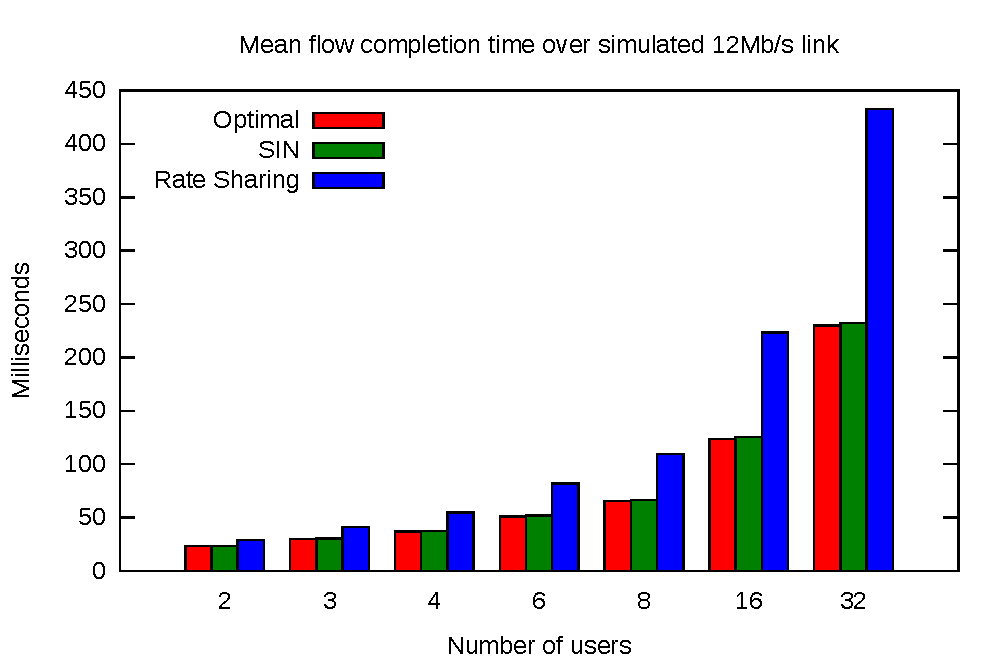
\includegraphics[width=\columnwidth]{plots/delay_over_srtf.pdf}
\caption{The blue line represents the efficient frontier, which here is defined entirely by the RemyCCs.}
\label{f:delay_over_srtf}
\end{figure}

\begin{figure}
%\vspace{\baselineskip}
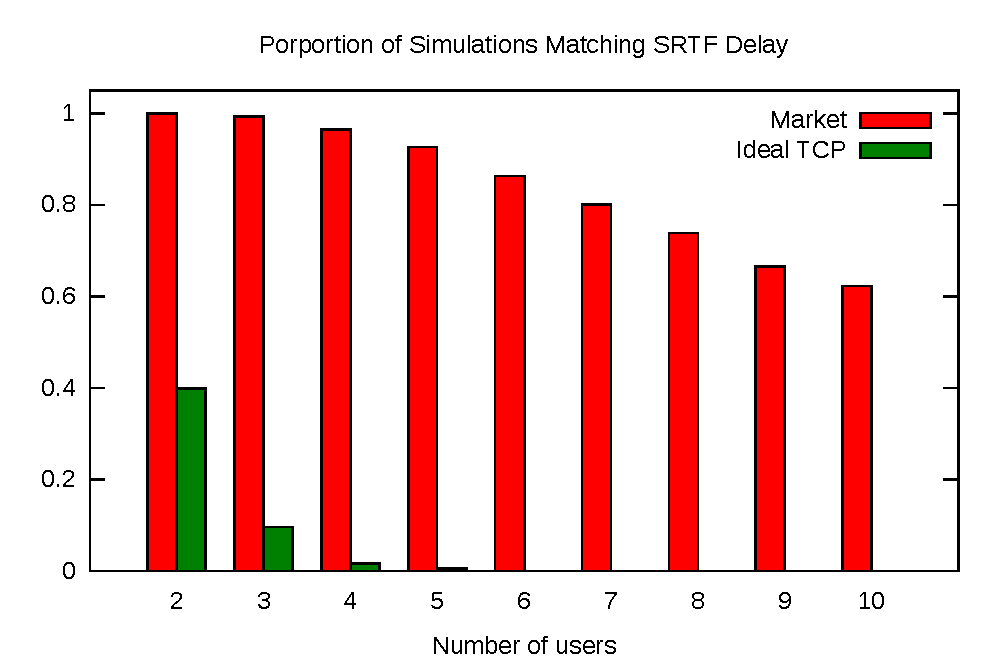
\includegraphics[width=\columnwidth]{plots/percent_match_srtf.pdf}
\caption{The blue line represents the efficient frontier, which here is defined entirely by the RemyCCs.}
\label{f:percent_match_srtf}
\end{figure}

Testing.

\section{Discussion and future work}
\label{sec:limits}

This position paper is a combination of several things:

\begin{enumerate}

\item a policy
argument that network neutrality ought to include neutrality towards
\textbf{customer} packets and a ``right to resell,''

\item an
architectural sketch about how that right could lead to 
Self-Incentivizing Networks and ameliorate some vexing problems, such
as the difficulty in deploying guaranteed services and mesh networks,
and

\item simulation experiments that suggest that a SIN market among
greedy endpoints can produce results at least as good as the status
quo (in fact, better than an idealized TCP), at least to the extent
those endpoints behave honestly.

\end{enumerate}

Each of these pieces would fairly be described as preliminary. On the
policy angle, we have not attempted an economic analysis to explain
whether consumer Internet access would cost more if retail ISPs were
forbidden to ban reselling.

On the architectural design and analysis, we have limited our
discussion to the case of scheduling a single hop and have not
discussed routing or topology-discovery problems at all, although we
view our work as complementary to related work that tackles these
issues~\cite{routebazaar15, esquivel09}.

In future work, we intend to show rigorously that the multiresolution
market satisfies a bounded incentive-compatibility
property, such that strategic bidders can only inflict a
logarithmically-bounded amount of pain or advantage for themselves. We
think the hierarchical nature of the market will make such a showing
possible, but have not simulated or proved anything about these
markets yet, beyond pencil-and-paper experiments.

We have not discussed the problem of ``cheating''---if anybody can be
an ISP-for-a-day and offer to convey packets, what stops somebody from
taking money for packets that they then drop? How can the system
punish this behavior? Others have dealt with this problem in the
context of mesh networking~\cite{onions14, torpath14, kadupul15}, and
we expect we will need to leverage similar solutions.

We expect that the first deployment of a self-incentivizing network
would be in a friendlier domain, such as the ``Local
sharing'' case from Section~\ref{ss:towards}, where some of these
challenging game-theoretic issues might be deferred.

\section{Conclusions}
While the 90's saw a large body of work on paid QoS and economically incentivized mesh networks were studied in the 2000's, what seemed like good and necessary ideas for the future success of the internet never caught on.
The internet has become even more ubiquitous today, but we believe its resource efficiency and potential to add value to the lives of it's users is being held back by the lack of routing options and ability for applications to express their needs.
%the same issues brought up in the QoS and ad hoc networking literature.
Cable internet service is monopolized by one provider in a large portion of the United States, the internet in developing countries is really bad (TODO somethign else), and video confrencing is still rarely a smooth experience.

We think the literature on application driven QoS and incentivized networks needs to be brought together and viewed holistically to [do great things]. We see application driven QoS and incentivized (mesh) networking as ideas that add value to each other and are most likely to succeed when implemented together.

We desired a more fluid and efficient internet. With real guaruntees of service instead of false promises. We see a future where mobile devices are constantly chosing the best routes to achieve a good user experience from all connectivity options around them.
We think a connectivity shortage should be magnet to entrepreneurs. When cell carriers have trouble supplying capacity during a parade in downtown San Francisco or an oppresive government shuts down the main internet sources, mobile-ad hoc neworks would spring up serendipitously to users when the demand exists and users should be able to seamlessly chose routes for communication and evaluate them on more than just bandwidth per dollar.

In this paper, we introduced...
A set of flow completion time users achieve near optimal mean flow duration over a shared link while compensating users of long flows to be pre-empted

%for pricing to reduce congestion software of users needs to adapt its behavior to dynamic pricing.

%things greg wants to have covered here or elsewhere:
%applications should define their own objectives.

%The interface we see to the users is as simple as: how much to spend per day/month, and something that lets people see how much money different applications are spending. If OS enforces reasonable limits, no runaway spending, only applications that can take more than their fair share, which is no different than situation today

%Other advanced network features such as caching and multicast could be served by a competetive market
\label{sec:conc}


\bibliographystyle{abbrv} 
\begin{small}
\bibliography{sin}
\end{small}
\label{last-page}

\end{document}
